\section{Results}\label{s:results}
A total of 3144 models have been evaluated along with the baselines and some other models reported in the literature for all datasets. The baseline (BL1) output for different datasets are shown in Table \ref{t:baselineoutput}. For all Adult datasets, SVM achieves the highest F-scores, i.e., 80.786, 81.363 and 78.177 for Adult(F), Adult(V) of MIMIC-II and Adult of MIMIC-III datasets respectively. On the other hand, NB achieves the highest scores, i.e., 65.45, 66.083 and 64.569, for Senior (F), Senior (B) of MIMIC-II and Senior of MIMIC-III datasets respectively.  

\begin{table}[h] 
	\centering \caption{Baseline $F_{wa}$ score of the datasets} 
	\begin{tabular}{|c|c|c|c|c|c|c|}\hline	
	Classifier & \multicolumn{4}{|c|}{MIMIC-II} & \multicolumn{2}{|c|}{MIMIC-III} \\\hline
	& Adult(F) & Adult(V) & Senior(F) & Senior(V) & Adult & Senior \\\hline
	J48 & 77.803 & 76.514 & 56.903 & 54.258 & 73.182 & 48.546 \\\hline
	NB & 77.922 & 79.175 & 65.45 & 66.083 & 77.072 & 64.569 \\\hline
	RF & 78.55 & 79.478 & 37.404 & 50.968 & 77.646 & 50.052 \\\hline
	SVM & 80.786 & 81.363 & 64.224 & 61.995 & 78.177 & 57.835 \\\hline
\end{tabular}
\label{t:baselineoutput}
\end{table}

Results of all experiments on these datasets are illustrated in several bar-charts in the following sections (Data corresponding to each of these bar-charts are also available in tabular format in the supplementary file).

\subsection{Results on MIMIC-II Adult Binary (F) dataset}

\begin{figure}[h] 
	\centering
	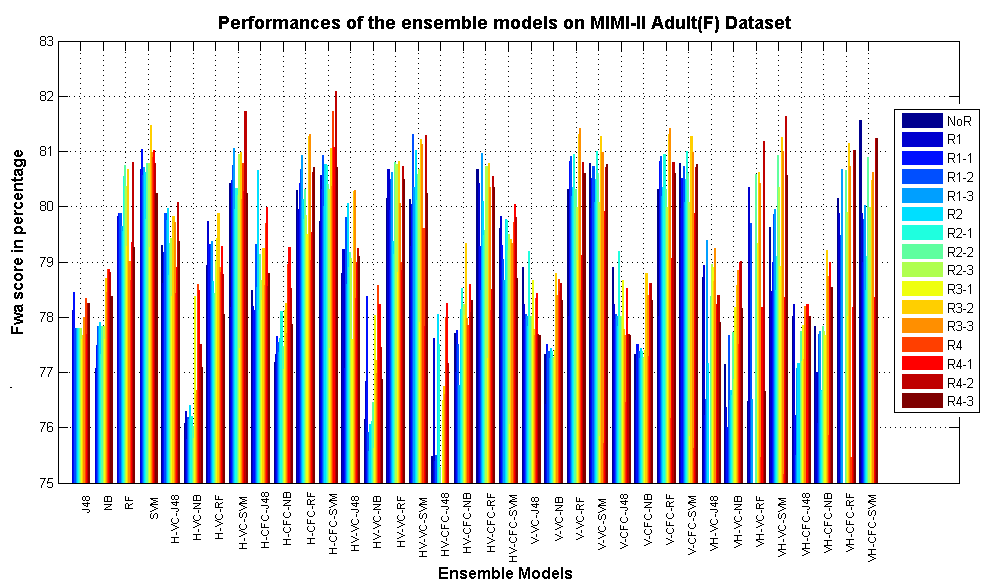
\includegraphics[scale=0.6]{fig/mimic2-adultk1f-full-table.png}
	\caption{$F_{wa}$ score of some experiments on MIMIC-II Adult Binary (F) dataset}
	\label{F:MIMIC2_AdultK1F_Table}
\end{figure}

Figure \ref{F:MIMIC2_AdultK1F_Table} represents the results of the experiments conducted on MIMIC-II Adult Binary (F) dataset. It is evident that after ranking SVM performs well compared to others. For example, when features are ranked by RandomForest and half of the total features are considered, SVM achieves a $F_{wa}$ score of 81.479. When features are compacted after ranking, SVM produces better results as compared to when feature compaction is applied without ranking. For example, SVM produces a $F_{wa}$ score of 81.479 when features are ranked - also by SVM; half of ranked features are selected; and Horizontal feature compaction is applied. The highest $F_{wa}$ score of 82.088 is produced by SVM when features are ranked by SVM; half of the total features are selected; horizontal FVC technique is applied; and finally, CFC is used as the ensemble method. This promising result may be attributed to several reasons, namely, focusing on (eliminating) some highly important and contributing (unimportant) features through ranking and selection, feature grouping and ensemble techniques. When a test instance is classified, it seems logical to use the model having the highest common features between them and thus the CFC approach contributed positively. More details are discussed in Section \ref{s:discussions}. 
 
It is also observed that RF also performs better as compared to J48 or NB for this dataset; in fact J48 and NB do not perform well on this dataset as compared to others. This may be attributed to the issue of how classifiers treat features in prediction. For example, NB treats features as independent, whereas SVM looks at the interactions among these to a certain degree. Naturally, features may be highly correlated for a patient with a disease thereby favouring the latter approach.   

\subsection{Results on MIMIC-II Adult Numeric (V) dataset}

\begin{figure}[h] 
	\centering 
	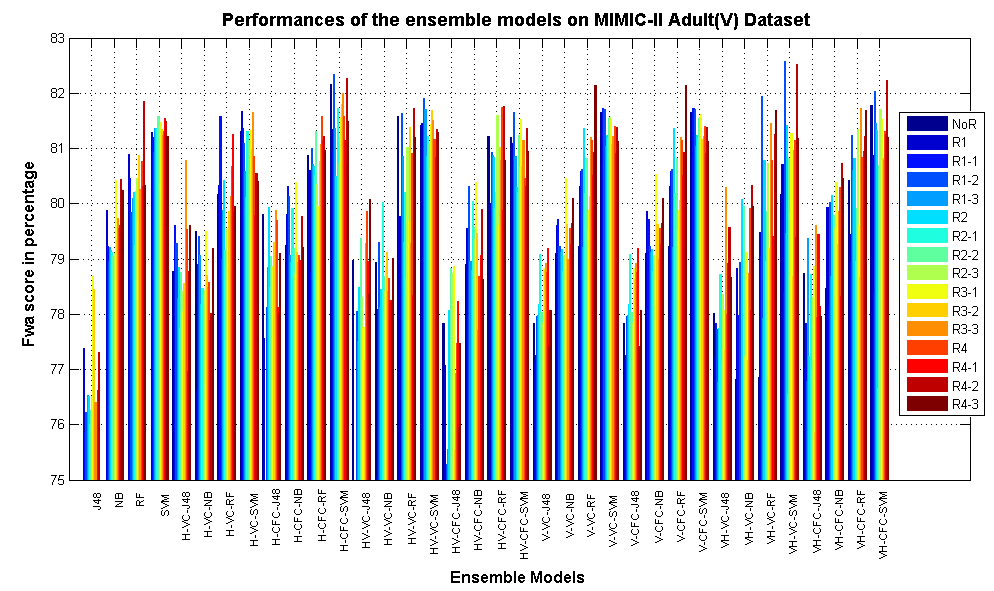
\includegraphics[scale=0.6]{fig/mimic2-adultk1v-full-table.png}
	\caption{$F_{wa}$ score of some experiments on MIMIC-II Adult Number (V) dataset}
	\label{F:MIMIC2_AdultK1V_Table}
\end{figure}

Figure \ref{F:MIMIC2_AdultK1V_Table} shows the results of the experiments conducted on MIMIC-II Adult Numeric (V) dataset. The results on this dataset indicate that SVM alone and its combination with other techniques produce better results. As an example, when features are ranked by SVM, half of the total features are selected, horizontal FVC is used and CFC is employed, then SVM as the classifier achieves a $F_{wa}$ score of 82.26. Changing the Horizontal FVC to Vertical (V) - Horizontal(H) FVC and CFC to VC achieves an even better $F_{wa}$ score of 82.512. But the highest  $F_{wa}$ score of 82.57 for SVM is achieved when features are ranked by Correlation ranker, half of the total features are selected, VH FVC are used and VC is applied as the ensemble technique. It is further observed that J48 and NB are not performing well on this dataset as compared to others using any combination of the techniques although RF observes improved results sometimes with different combinations.    

\subsection{Results on MIMIC-II Senior Binary (F) dataset}

\begin{figure}[h] 
	\centering 
	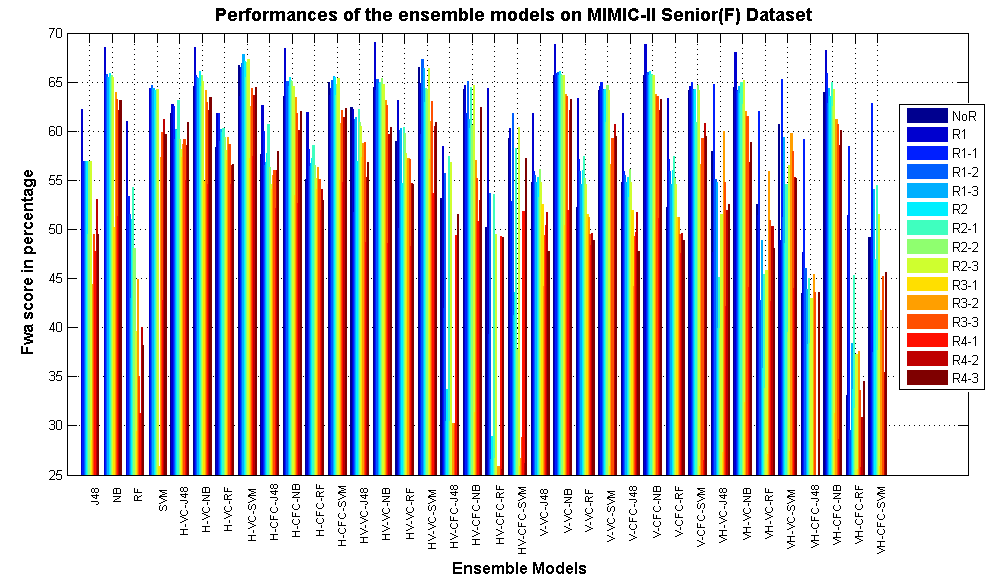
\includegraphics[scale=0.6]{fig/mimic2-seniork1f-full-table.png}
	\caption{$F_{wa}$ score of some experiments on MIMIC-II Senior Binary(F) dataset}
	\label{F:MIMIC2_SeniorK1F_Table}
\end{figure} 

Figure \ref{F:MIMIC2_SeniorK1F_Table} displays the results of the experiments performed on MIMIC-II Senior Binary (F) dataset. Evidently, NB combined with other techniques performs better for this dataset. As an instance, when features are ranked by InfoGain ranker, ${1/4}$th of the total features are selected, NB achieves 68.502 as the $F_{wa}$ score. Just after applying a vector compaction technique following the previous process, the result improves. For example, $F_{wa}$ score of 68.808 is achieved when Vertical(V) vector compaction technique is used with VC ensemble technique. However, the highest $F_{wa}$ score of 69.014 is achieved by NB when features are ranked by InfoGain ranker, ${1/4}$th of the total features are selected, Horizontal(H)-Vertical(V) FVC is used and VC is applied as the ensemble technique. J48 and RF fail to do well on this dataset as compared to others using any combination of the techniques. SVM sometimes has performed better in comparison with these two.    

\subsection{Results on MIMIC-II Senior Numeric (V) dataset}

\begin{figure}[h] 
	\centering 
	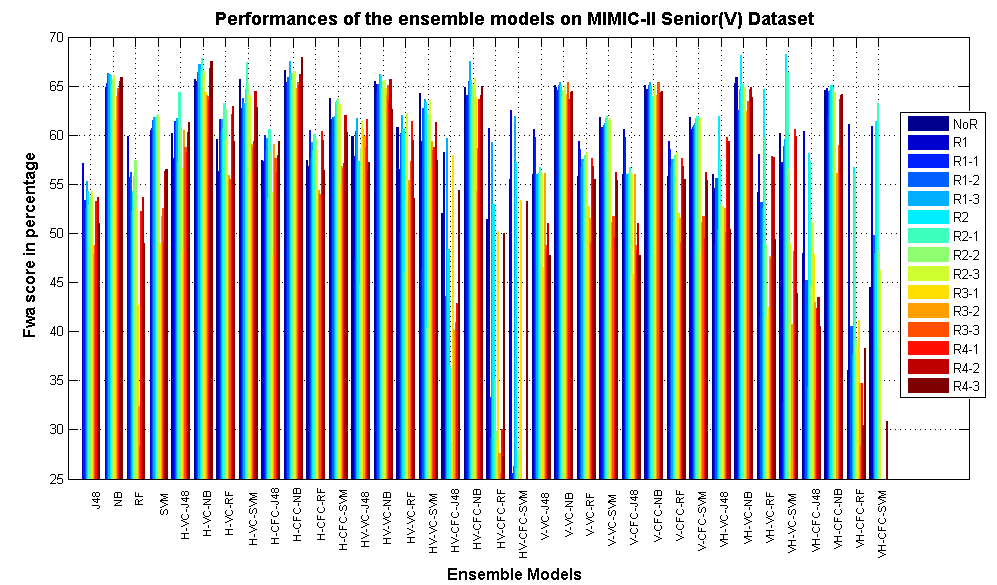
\includegraphics[scale=0.6]{fig/mimic2-seniork1v-full-table.png}
	\caption{$F_{wa}$ score of some experiments on MIMIC-II Senior Numeric (V) dataset}
	\label{F:MIMIC2_SeniorK1V_Table}	
\end{figure} 

Figure \ref{F:MIMIC2_SeniorK1V_Table} shows the results of the experiments conducted on MIMIC-II Senior Numeric (V) dataset. As is evident from the results, NB, combined with other techniques, has achieved better results. For example, when features are ranked by Correlation ranker, half of the total features are selected and Horizontal FVC is used along with VC as the ensemble technique, NB scores 67.806 (as $F_{wa}$ score). However, sometimes SVM combined with other techniques performs better. The highest $F_{wa}$ score of SVM, i.e., 68.215 is achieved when features are ranked by Correlation ranker, ${1/4}$th of the total features are selected, Vertical(V)-Horizontal(V) FVC are used and VC is applied as the ensemble technique. J48 and RF are not performing well on this dataset as compared to others using any combination of the techniques.
 
\subsection{Results on MIMIC-III Adult dataset}
\begin{figure}[h] 
	\centering
	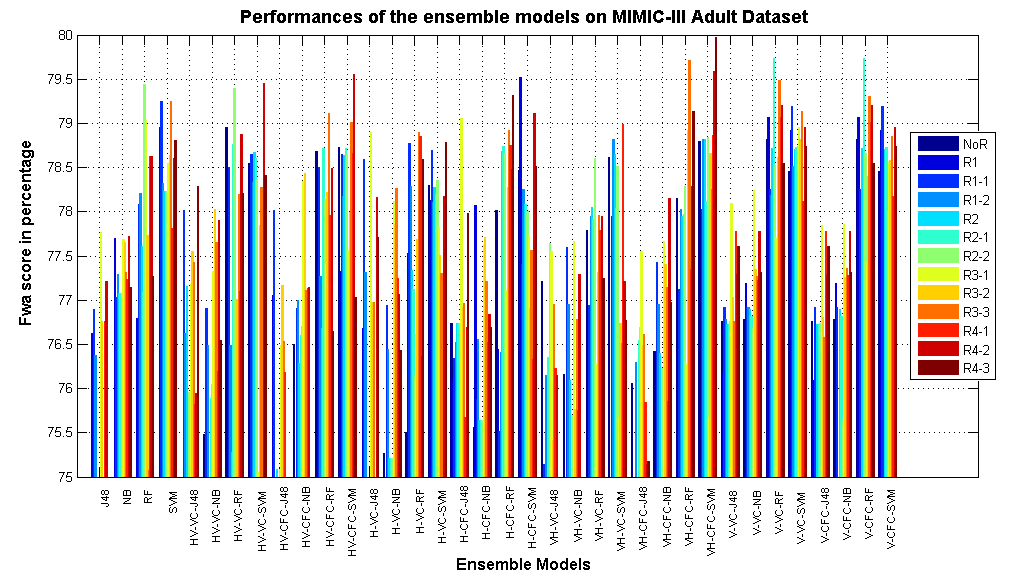
\includegraphics[scale=0.6]{fig/mimic3-adult24hrs-full-table.png}
	\caption{$F_{wa}$ score of some experiments on MIMIC-III Adult dataset}
	\label{F:MIMIC3_Adult24hrs_Table}
\end{figure} 

Figure \ref{F:MIMIC3_Adult24hrs_Table} presents the results of the experiments done on MIMIC-III Adult dataset. The results on this dataset hint that SVM combined with other techniques produces the most competitive results. As an example, when features are ranked by InfoGain ranker, ${3/4}$th of the total features are selected and Horizontal FVC is used along with CFC as the ensemble technique, SVM achieves 79.518 as the $F_{wa}$ score. RF also is observed to have performed well. The highest $F_{wa}$ score of 79.975, produced by SVM is achieved when features are ranked by SVM ranker, ${3/4}$th of the total features are selected, Vertical(V)-Horizontal(V) FVC are used along with CFC ensemble technique. %J48 and NB also perform well on this dataset compared to others using any combination of the techniques.

\subsection{Results on MIMIC-III Senior dataset}

\begin{figure}[h] 
	\centering 
	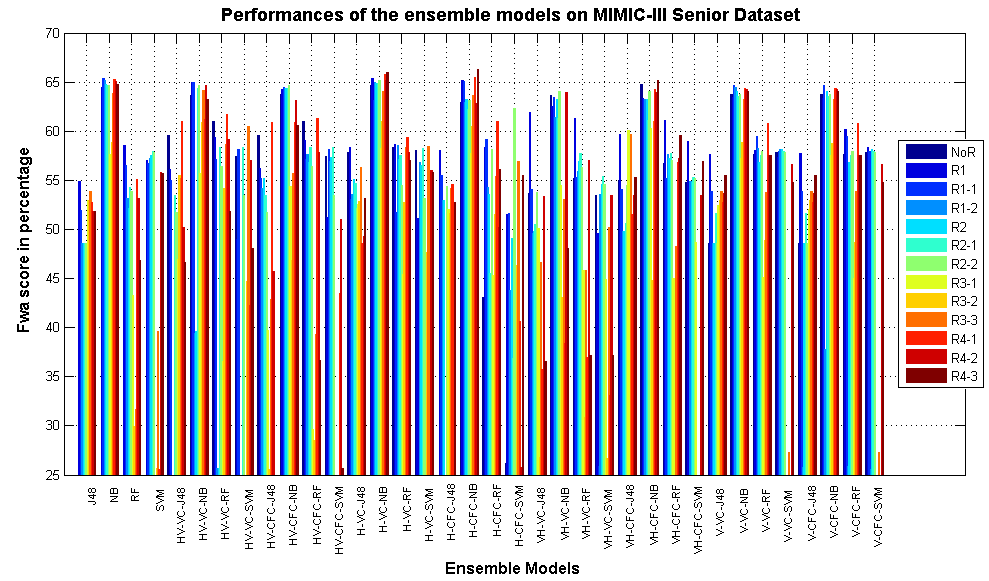
\includegraphics[scale=0.6]{fig/mimic3-senior24hrs-full-table.png}
	\caption{$F_{wa}$ score of some experiments on MIMIC-II Senior dataset}
	\label{F:MIMIC3_Senior24hrs_Table}
\end{figure} 

Figure \ref{F:MIMIC3_Senior24hrs_Table} demonstrates the results of the experiments conducted on MIMIC-III Adult dataset. The results on this dataset show that NB combined with other techniques produces better results. As an example, when features are ranked by SVM ranker,  ${3/4}$th of the total features are selected and Horizontal FVC is used along with VC as the ensemble technique, NB achieves 65.945 as the $F_{wa}$ score. The highest $F_{wa}$ score of 66.333 produced by NB, is achieved when features are ranked by SVM ranker, ${3/4}$th of the total features are selected, Horizontal(V) FVC are used along with CFC as the ensemble technique. Unfortunately other classifiers did not perform well here.

\subsection{Summary comparison with baselines and state of the arts}

\begin{figure}[h] 
	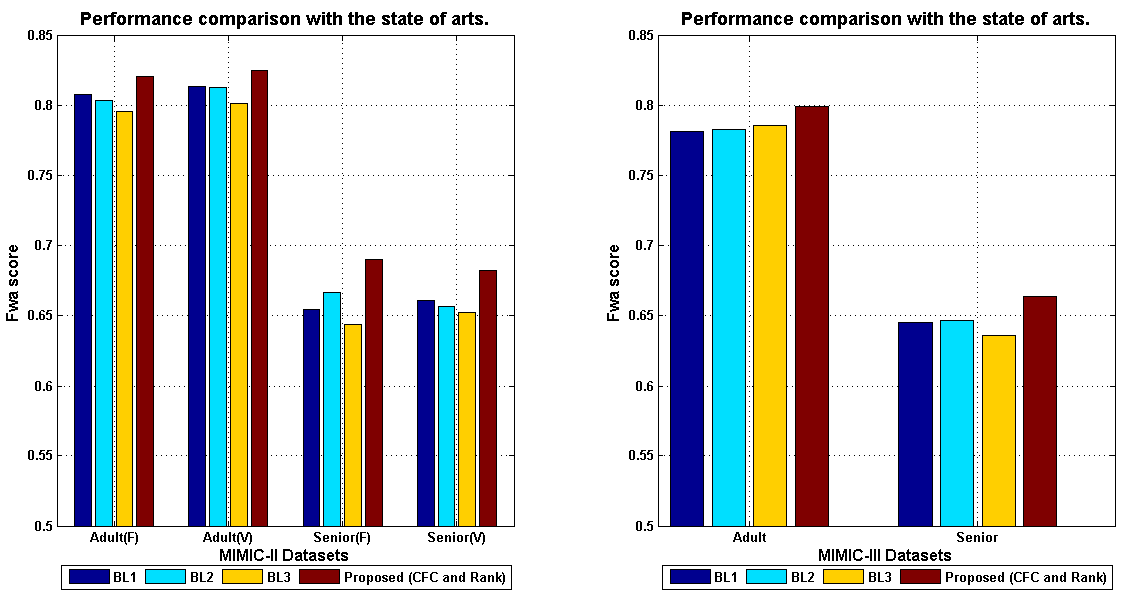
\includegraphics[scale=0.5]{fig/comparison-with-state-of-arts.png}
	\centering \caption{Performance comparison the proposed method with the state of the arts in terms of $F_{wa}$ score. Here BL1 means when no preprocessing technique is applied; BL2 is the technique proposed by the study \cite{mehedy-masud:2017:fvc}; And BL3 is the method introduced in the study \cite{mehedy-masud:2018:frmwrk}. The highest scored ensemble models seen in Figures \ref{F:MIMIC2_AdultK1F_Table} $-$ \ref{F:MIMIC3_Senior24hrs_Table} for each dataset are compared here with the state of the arts.}
	\label{F:comparison_with_state_of_art}
\end{figure}

% Model - i - information
%-----dataset------ Higest - Total
%MIMIC-II-Adult(F) - 187 - 572
%MIMIC-II-Adult(V) - 496 - 572
%MIMIC-II-Senior(F) - 206 - 536
%MIMIC-II-Senior(V) - 498 - 536
%MIMIC-III-Adult - 360 - 464
%MIMIC-III-Senior - 230 - 464
%
%--------------------Total - 3144
%

Figure \ref{F:comparison_with_state_of_art} presents the performance comparison of the proposed technique with the state of the arts, such as, the results produced by the techniques of \cite{mehedy-masud:2017:fvc} (i.e., BL2) and \cite{mehedy-masud:2018:frmwrk} (i.e., BL3) in terms of $F_{wa}$ score. The left panel and the right panel of Figure \ref{F:comparison_with_state_of_art} show the performance of the highest scored model comparing with all previous baselines for each of MIMIC-II and MIMIC-III datasets respectively. For MIMIC-II datasets, Model$_\mathrm{187}^\mathrm{AF-R4-2HCFCSVM}$, Model$_\mathrm{496}^\mathrm{AV-R1-2VHVCSVM}$, Model$_\mathrm{206}^\mathrm{SF-R1HVVCNB}$, and Model$_\mathrm{498}^\mathrm{SV-R2VHVCSVM}$ are the highest scored models for Adult Binary (F), Adult Numeric (V), Senior Binary (F) and Senior Numeric (V) datasets respectively. For MIMIC-III datasets, Model$_\mathrm{360}^\mathrm{AV-R4-3VHCFCSVM}$ and Model$_\mathrm{230}^\mathrm{SV-R4-3HCFCNB}$ are the highest scored models for Adult and Senior datasets respectively. Their $F_{wa}$ scores are compared with all previous baselines in Figure \ref{F:comparison_with_state_of_art}. 

\textcolor{blue}{Table \ref{t:Summary_of_results_with_all_baselines2} presents the results of this study in terms of  Accuracy, Precision, Recall, and F1 score comparing with baselines for each dataset. For each case, it is clearly observed that our model is doing better compared to all the baselines.}

\begin{table}[h] 
	\tiny %\small
	\centering \caption{\textcolor{blue}{Accuracy, Precision, Recall, and F1 score of this study comparing with baselines}} 
	\begin{tabular}{|p{1.5cm}|p{0.6cm}|p{0.6cm}|p{0.6cm}|p{0.6cm}|p{0.6cm}|p{0.6cm}|p{0.6cm}|p{0.6cm}|p{0.6cm}|p{0.6cm}|p{0.6cm}|p{0.6cm}|p{0.6cm}|p{0.6cm}|p{0.6cm}|p{0.6cm}|}\hline	
		& \multicolumn{4}{|c|}{BL1} & \multicolumn{4}{|c|}{BL2} & \multicolumn{4}{|c|}{BL3} & \multicolumn{4}{|c|}{This study} \\\hline	
		DataSet	& Acc. & Pre. & Rec. & F1 & Acc. & Pre. & Rec. & F1 & Acc. & Pre. & Rec. & F1 & Acc. & Pre. & Rec. & F1 \\\hline	
		MIMIC-II Adult (F) & 81.296 & 70.309 & 68.203 & 69.119 & 81.094 & 69.856 & 67.186 & 68.294 & 82.174 & \textbf{72.647} & 62.385 & 64.633 & \textbf{82.512} & 72.442 & \textbf{70.363} & \textbf{71.287} \\\hline 
		MIMIC-II Adult (V) & 81.634 & 71.022 & 69.815 & 70.375 & 81.499 & 70.850 & 69.985 & 70.395 & 82.512 & 73.412 & 63.360 & 65.754 & \textbf{83.255} & \textbf{73.797} & \textbf{70.190} & \textbf{71.672} \\\hline  
		MIMIC-II Senior (F) & 65.681 & 68.189 & 67.689 & 65.635 & 66.683 & 68.228 & 68.200 & 66.683 & 64.679 & 67.263 & 66.725 & 64.621 & \textbf{69.038} & \textbf{68.333} & \textbf{68.276} & \textbf{68.303} \\\hline
		MIMIC-II Senior (V) & 67.184 & 66.831 & 64.684 & 64.705 & 66.232 & 65.387 & 64.428 & 64.557 & 66.483 & 66.108 & 63.846 & 63.783 & \textbf{68.136} & \textbf{67.541} & \textbf{67.716} & \textbf{67.603} \\\hline 
		MIMIC-III Adult & 79.068 & 66.022 & 63.502 & 64.486 & 79.406 & 66.669 & 64.094 & 65.110 & 79.338 & 66.525 & 63.925 & 64.944 & \textbf{80.824} & \textbf{69.268} & \textbf{66.126} & \textbf{67.369} \\\hline
		MIMIC-III Senior & 64.930 & 63.962 & 63.398 & 63.508 & 63.577 & 62.878 & 62.973 & 62.914 & 64.429 & 63.429 & 62.478 & 62.542 & \textbf{66.633} & \textbf{65.774} & \textbf{65.214} & \textbf{65.351} \\\hline  
		
	\end{tabular}
	\label{t:Summary_of_results_with_all_baselines2}
\end{table}

\begin{figure}[h] 
	\centering 
	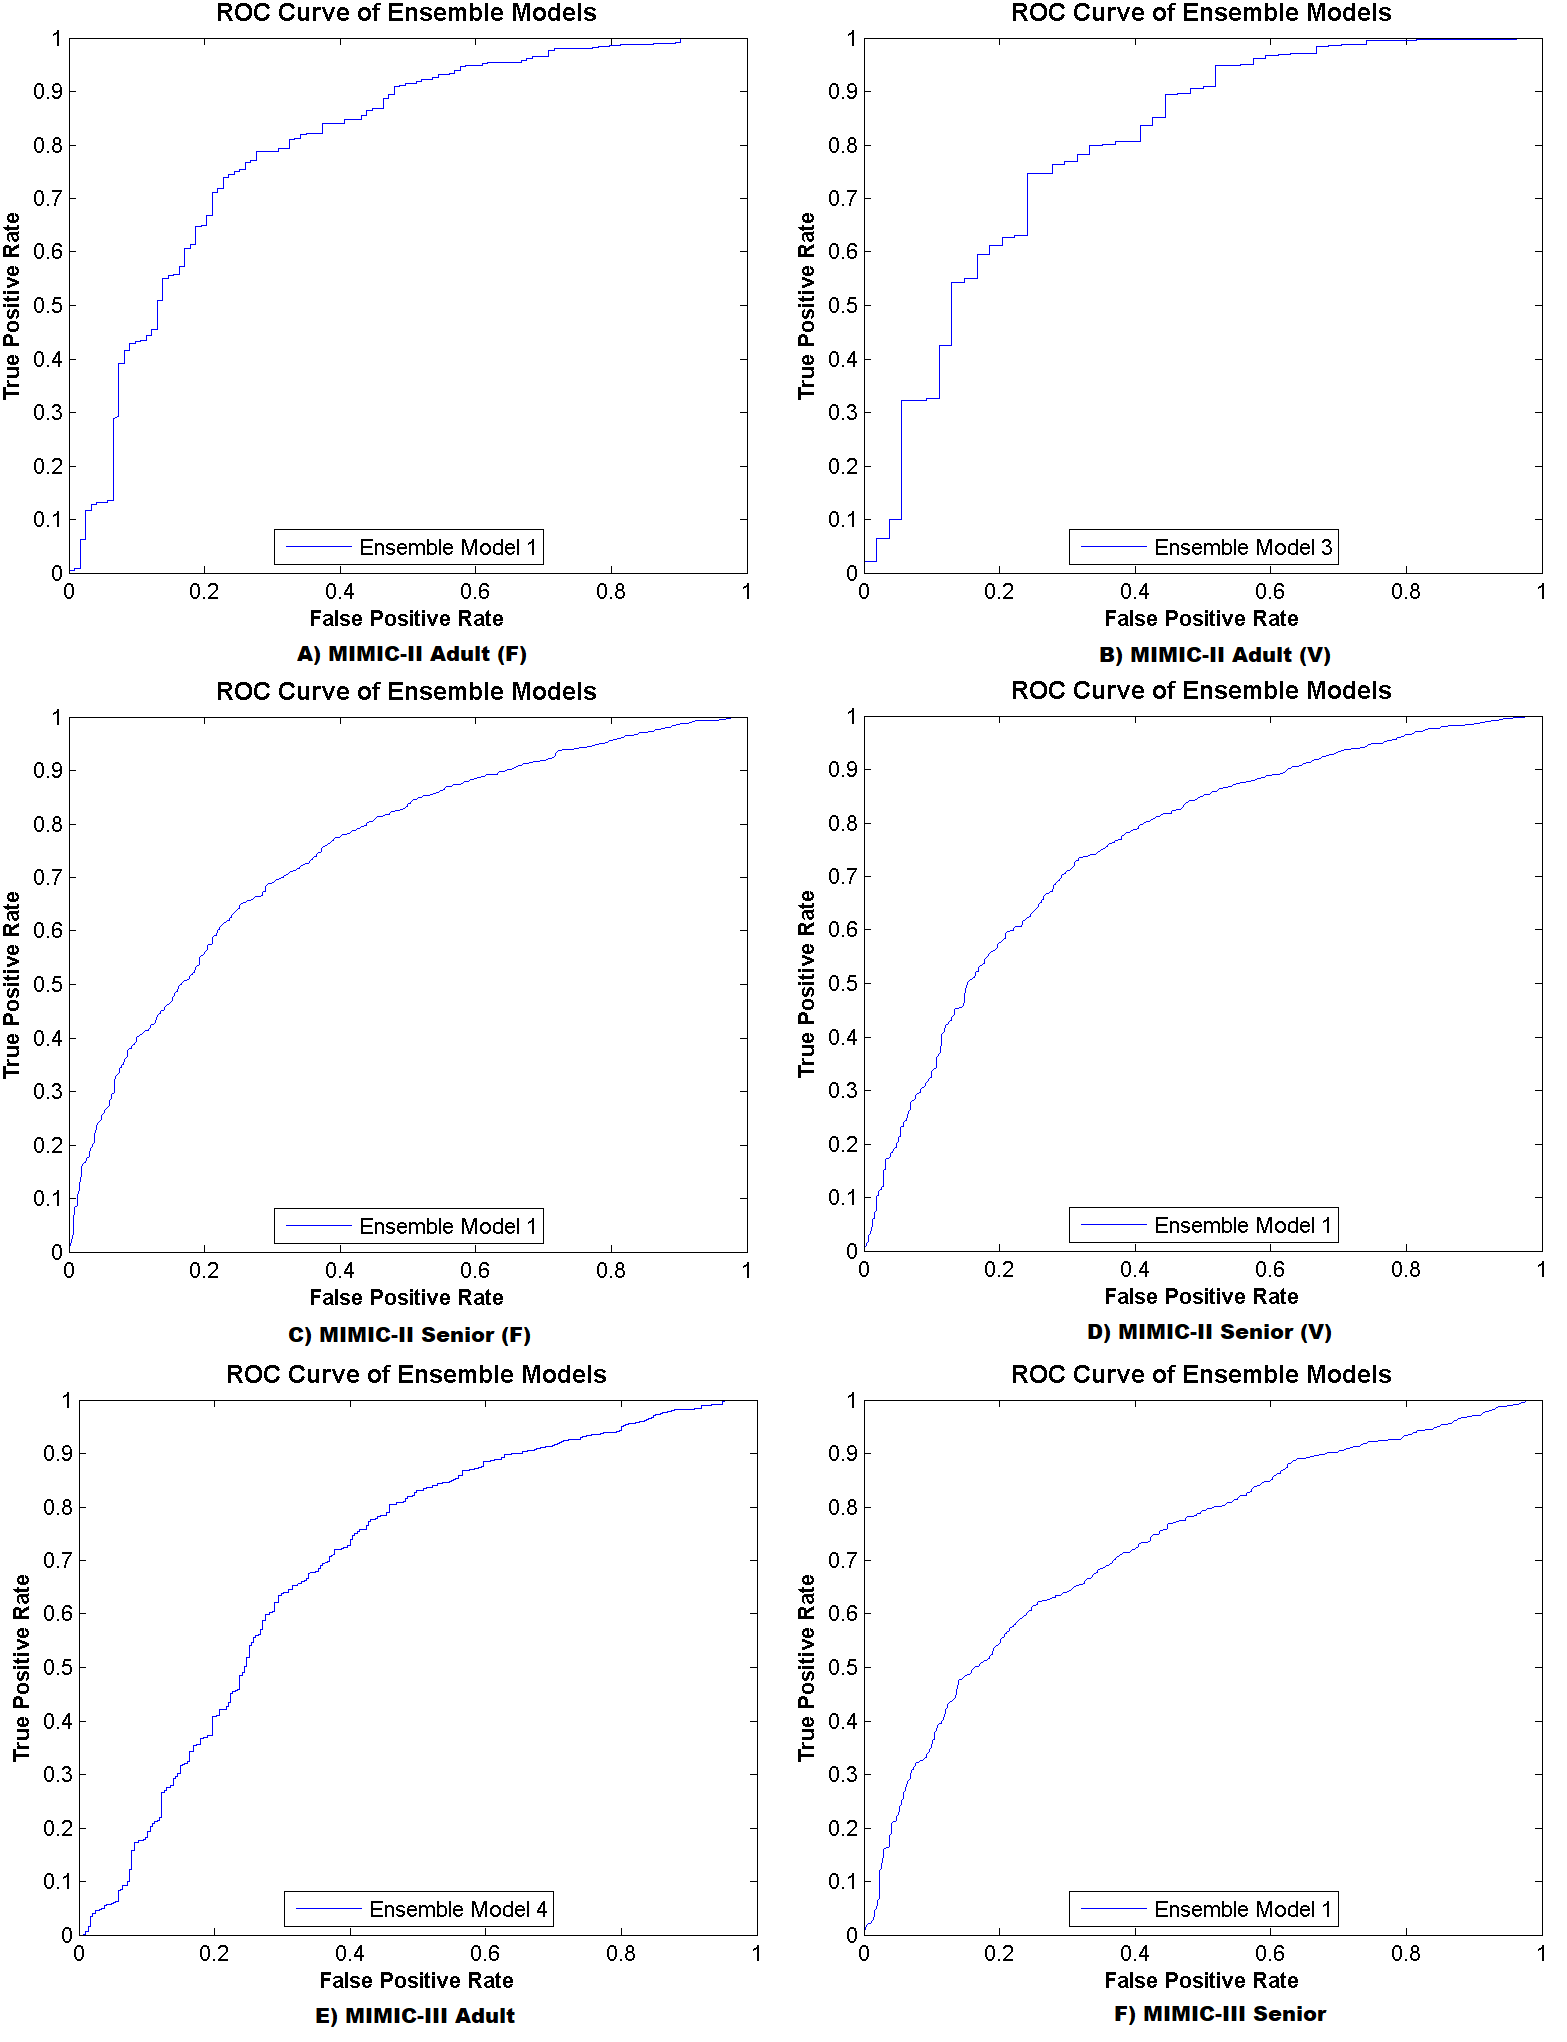
\includegraphics[scale=0.25]{fig/ROC-top.png}
	\caption{ROC Curve of some ensemble models for each dataset}
	\label{F:ROC}
\end{figure} 

In addition to the above results, Figure \ref{F:ROC} presents some ROC curves of some ensemble models which are used in this study for each dataset. Each of these curves is above of the 45-degree diagonal axes and have a tendency towards the top-left corner. These indicate that these models have capability for doing better.      
      
Table \ref{t:Summary_of_results_with_all_baselines} presents the summary of the results of the proposed techniques along with other baselines, i.e, BL1, BL2 and BL3. From these results it is evident that for every dataset, the proposed techniques are producing better results compared to all previous baselines.   

\begin{table}[h] 
	\centering \caption{Summary of the results comparing with baselines in terms of $F_{wa}$ score} 
	\begin{tabular}{|p{0.8cm}|p{1cm}|p{0.6cm}|p{0.8cm}|p{0.6cm}|p{0.8cm}|p{0.6cm}|p{0.8cm}|p{5.0cm}|p{1cm}|p{0.7cm}|}\hline	
		Age group type & Data Type & BL1 & $F_{wa}$ of BL1 & BL2 & $F_{wa}$ of BL2 & BL3 & $F_{wa}$ of BL3 & Proposed (CFC and Rank) & $F_{wa}$ of the proposed & $F_{wa}$ (+/-) over BL3 \\\hline		
		
		\multicolumn{11}{|c|}{\textbf{MIMIC-II}} \\\hline
		Adult & Binary (F) &	SVM	& 80.786 & SVM	& 80.414 &	SVM & 79.618 & First ranking, then H grouping-CFC is used in ensemble (Alg: SVM)	& \textbf{82.088}	& 2.47 \\\hline
		Adult & Numeric (V)	& SVM &	81.363 & SVM & 81.303 & SVM & 80.166 &	First ranking then VH grouping and then VC is used in ensemble (Alg: SVM) &	\textbf{82.57} & 2.404 \\\hline
		Senior & Binary (F) & NB & 65.45 & SVM & 66.671 & NB & 64.41 & First ranking, then HV grouping  and then VC is used in ensemble  (Alg: NB) & \textbf{69.014} &  4.604 \\\hline
		Senior & Numeric (V) & NB & 66.083 & NB & 65.692 & NB & 65.239 & First ranking then VH grouping and then VC is used in ensemble (Alg: SVM) &	\textbf{68.215} & 2.976 \\\hline
		
		\multicolumn{11}{|c|}{\textbf{MIMIC-III}} \\\hline	
		Adult & 24hrs & SVM & 78.177 & SVM & 78.546 & SVM & 78.459 & First ranking then VH grouping and then CFC is used in ensemble (Alg: SVM) &	\textbf{79.975} &  1.516 \\\hline
		Senior & 24hrs & NB & 64.569 & NB & 63.644 & NB & 63.780 & First ranking then H grouping and then CFC is used in ensemble (Alg: NB) &	\textbf{66.333}	& 2.553 \\\hline
		
	\end{tabular}
	\label{t:Summary_of_results_with_all_baselines}
\end{table}



